\documentclass[conference]{assets/latex/IEEEtran}
\IEEEoverridecommandlockouts

\usepackage{amsmath,amssymb,amsfonts}
\usepackage{graphicx}
\usepackage{textcomp}
\usepackage{xcolor}
\usepackage{booktabs}
\usepackage[backend=biber,style=numeric]{biblatex}
\addbibresource{assets/latex/report.bib}

\graphicspath{{assets/latex/}}

\begin{document}

\title{CS6524 Computer Vision Lab. 2\\ Camera Calibration and Stereo Vision}

\author{\IEEEauthorblockN{Cormac Shannon}
\IEEEauthorblockA{\textit{ID 23366303} \\
\textit{University of Limerick}}
\and
\IEEEauthorblockN{Eddie Phelen}
\IEEEauthorblockA{\textit{ID 23397179} \\
\textit{University of Limerick}}
\and
\IEEEauthorblockN{Ellice Nelson}
\IEEEauthorblockA{\textit{ID 23371323} \\
\textit{University of Limerick}}
}

\maketitle

\begin{abstract}
This report describes a pipeline that calibrates a phone camera from a checkerboard video and then uses those intrinsics to estimate the depth of a scene from a single moving camera. Three phones were calibrated (Samsung Galaxy Z Fold6, iPhone 15 and iPhone 15 Pro), with mean reprojection errors between 0.12 and 0.41\,px. For depth, the relative pose between two frames of a scene video is recovered from SIFT matches and the essential matrix, and the pair is then rectified and matched with semi-global block matching. Our first working version produced depth for only 5 frame pairs across all three scenes. Two problems were responsible: a default threshold in \texttt{recoverPose} that discarded most of the scene, and the ambiguity between a small pan and a small sideways slide. With both addressed, 212 pairs produce depth maps whose ordering is correct in every scene. The weakest part of the pipeline remains the absolute scale, which relies on assuming the phone moves at a steady speed.
\end{abstract}

\section{Introduction}
A camera's intrinsic matrix $K$ describes how it projects points in the world onto its image plane. Once $K$ is known, the motion of the camera between two frames can be recovered from the frames alone, and two frames taken from slightly different positions can be treated as a stereo pair. In this lab, each member recorded a calibration video and a scene video with their own phone, with the goal of producing a depth video of each scene in centimetres.

The project has the following objectives:
\begin{enumerate}
\item Calibrate each phone camera from 20 frames of a checkerboard video and report $K$, the distortion coefficients $D$ and the reprojection error.
\item Estimate the relative pose $(R, t)$ between frames of a scene video.
\item Rectify frame pairs, compute dense disparity, and convert it to depth in centimetres.
\end{enumerate}

\section{Methodology}

\subsection{Recording and Pre-processing}
Each member recorded a calibration video, in which the phone is held still and the board is moved, and a scene video, in which the scene is still and the phone slides sideways. All videos pass through the same function, which resizes them to fit within $640\times360$. It is important to note that the function ignores the rotation flag stored in the video container. Phones record in their sensor's orientation and only mark the file as rotated, so honouring that flag could give the scene frames a different pixel layout from the one $K$ was estimated in.

\subsection{Calibration}
The printed board has $9\times6$ squares, which gives $8\times5$ inner corners rather than the $9\times6$ inner grid described in the lab brief. The corners are placed at $(i s, j s, 0)$ with $s = 2.5$\,cm, so every 3D result downstream is in centimetres. To get a variety of board poses, the video is split into 20 equal time windows and the sharpest frame with a visible board (by variance of the Laplacian) is taken from each.

Corners are detected with \texttt{findChessboardCornersSB}, OpenCV's sector-based detector, which is sub-pixel accurate on its own. We also tried \texttt{findChessboardCorners} followed by \texttt{cornerSubPix}, however, on one washed-out frame from camera 01 this misplaced two corners, giving a 1.2\,px error for that frame against 0.12\,px with the sector-based detector. The corners from all frames are then passed to \texttt{calibrateCamera}~\cite{zhang2000}. Table~\ref{tab:calib} lists the results; the error is the mean distance between each detected corner and its reprojection.

\begin{table}[t]
\caption{Calibration results (pixels, $640\times360$; skew is 0). 01: Galaxy Z Fold6, 02: iPhone 15, 03: iPhone 15 Pro}
\label{tab:calib}
\centering
\setlength{\tabcolsep}{3pt}
\begin{tabular}{@{}lccccc@{}}
\toprule
Cam. & $f_x, f_y$ & $c_x, c_y$ & $k_1, k_2, k_3$ & $p_1, p_2$ & err. \\
\midrule
01 & 552.0, 552.0 & 321.0, 169.4 & 0.05, $-$0.30, 0.42 & $-$.005, .001 & 0.12 \\
02 & 624.9, 623.3 & 324.4, 185.2 & 0.37, $-$2.32, 5.37 & .002, .000 & 0.41 \\
03 & 564.5, 565.0 & 315.9, 168.6 & 0.27, $-$1.21, 2.56 & $-$.011, $-$.002 & 0.32 \\
\bottomrule
\end{tabular}
\end{table}

\begin{figure*}[t]
\centering
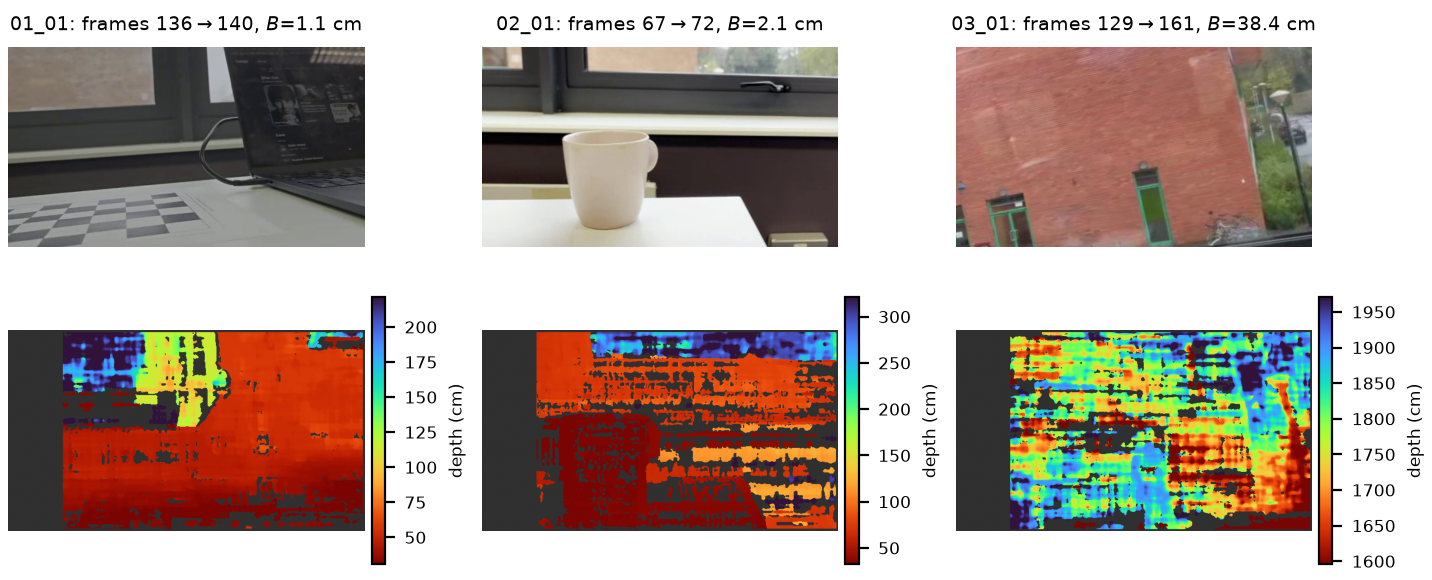
\includegraphics[width=\textwidth]{depth_examples.png}
\caption{Rectified first frame (top) and estimated depth (bottom) for one pair from each scene. Grey pixels have no valid disparity. Each scene has its own colour scale (5th to 95th percentile).}
\label{fig:depth}
\end{figure*}

\subsection{Relative Pose Estimation}
SIFT~\cite{lowe2004} keypoints are detected in each frame and matched by brute force, keeping matches that pass Lowe's ratio test (0.75). At $640\times360$ the default contrast threshold only found around 250 keypoints per frame, so it was lowered from 0.04 to 0.02, which roughly doubled that number. The matched points are undistorted and passed to \texttt{findEssentialMat}, which estimates the essential matrix $E$ with the 5-point algorithm~\cite{nister2004} inside RANSAC.

We chose to estimate $E$ directly rather than estimating the fundamental matrix $F$ and computing $E = K^\top F K$. Since $K$ is already known, $E$ has only 5 unknowns compared to 7 for $F$, and on scene 01 the direct estimate gave more consistent translation directions between neighbouring pairs (0.90 against 0.79 agreement). \texttt{recoverPose} then decomposes $E$ into $R$ and a unit-length $t$, choosing whichever of the four possible decompositions places the most points in front of both cameras.

A pair of consecutive frames is a poor stereo pair: the features move less than a pixel between them, which leaves almost no parallax to work with. Instead, for every frame we search forward for the first frame where the matched features have moved at least 10\,px (median), up to 90 frames ahead. A pose is rejected if the features barely moved (under 3\,px), if fewer than half of the RANSAC inliers lie in front of both cameras, or if it fails the consistency check described in Section~\ref{sec:discussion}.

\begin{figure}[t]
\centering
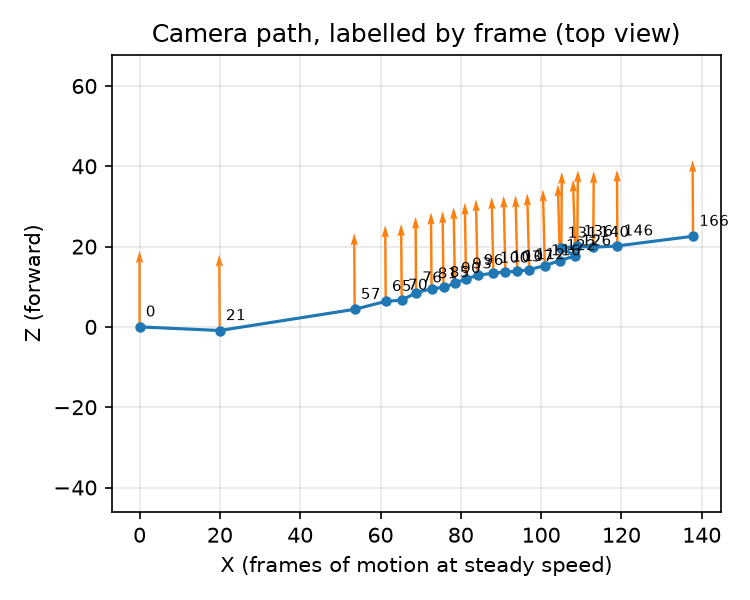
\includegraphics[width=0.7\columnwidth]{trajectory_01_01.png}
\caption{Camera path of scene 01\_01 from top down, built by chaining frame pairs. Each step is scaled by its gap in frames; arrows show the viewing direction.}
\label{fig:traj}
\end{figure}

\subsection{Dense Depth Estimation}
Each accepted pair is rectified with \texttt{stereoRectify}, \texttt{initUndistortRectifyMap} and \texttt{remap}, so that matching points lie on the same image row. Pairs that rotate more than $10^\circ$, or whose rectification would rescale the image by more than a factor of two (which happens when the phone moves forward rather than sideways), are skipped. Some of scene 02 was filmed moving the phone vertically; for these pairs both rectified images are transposed, so that the vertical epipolar lines become rows and the same matcher can be used.

Disparity is computed with StereoSGBM~\cite{hirschmuller2008} using a $7\times7$ window and 96 disparity levels, with a left--right consistency check and speckle filtering, followed by a $5\times5$ median filter. Depth is then
\begin{equation}
Z = \frac{f B}{d} = \frac{-P_2[0,3]}{d},
\end{equation}
where $P_2$ is the second rectified projection matrix, whose last column already contains the product $f B$ (we use $P_2[1,3]$ for vertical pairs). The output video shows each pair's depth with a colour bar in centimetres; frames without a usable pair keep showing the most recent depth map.

\subsection{Recovering Scale}
\texttt{recoverPose} only returns the direction of $t$, not its length, so the baseline $B$ cannot be recovered from the video itself. The phones' video metadata holds no subject distance or motion data either. We therefore assume the phone moves at a steady speed $v$ through each scene, giving $B = v\,(t_2 - t_1)$, and estimate $v$ from something of known size.

For scene 01\_01 this is a measurement. The calibration board was left on the desk, and after upscaling the frames by $2\times$ it is detected in five frames between 90 and 107. Using \texttt{solvePnP}, the camera is 22--35\,cm from the board and moves 4.6\,cm over those 17 frames, so $v = 0.27$\,cm/frame. The other two scenes rely on typical sizes. In 02\_01 the mug is 152\,px tall, which for a 9.5\,cm mug puts it 39\,cm away (its width gives 38.5\,cm). In 03\_01 the building's storeys repeat every 95\,px and its doors are around 60\,px tall; assuming 3\,m storeys and 2\,m doors puts the wall 17.8--18.8\,m away. For these two scenes $v$ is chosen so that the object comes out at that distance, taking the median over the pairs within 8 frames of the reference frame, giving 0.42 and 1.2\,cm/frame respectively.

\section{Results}

\begin{table}[t]
\caption{Pose and depth per scene}
\label{tab:scenes}
\centering
\setlength{\tabcolsep}{4pt}
\begin{tabular}{@{}lccccc@{}}
\toprule
Scene & frames & poses & depth (first version) & median gap & coverage \\
\midrule
01\_01 & 173 & 77 & 75 (2) & 4 & 0.57 \\
02\_01 & 281 & 138 & 111 (1) & 14 & 0.40 \\
03\_01 & 205 & 54 & 26 (2) & 52 & 0.57 \\
\bottomrule
\end{tabular}
\end{table}

Table~\ref{tab:scenes} shows how many frame pairs survive each stage of the pipeline, where coverage is the median fraction of pixels in a depth map that have a valid depth. Fig.~\ref{fig:depth} shows one pair from each scene. In all three the depth ordering is correct and the values are plausible: in 01\_01 the desk is 30--50\,cm away and the window 1--2\,m; in 02\_01 the mug is around 40\,cm away with the window frame behind it; and in 03\_01 the building wall forms a nearly flat plane at 16--19\,m, with the trees and car park further back. On scene 01\_01, 75 of the 77 accepted poses have $t \approx (-1, 0, 0)$, consistent with the phone sliding to the right, and chaining the pairs together gives a smooth sideways path (Fig.~\ref{fig:traj}).

\section{Discussion and Failure Analysis}\label{sec:discussion}

\textbf{Points at infinity.} The first version of the pipeline accepted only 2, 1 and 2 pairs (Table~\ref{tab:scenes}), even though feature matching was working well. The cause was \texttt{recoverPose}: it only counts a point as being in front of the cameras if its depth is less than \texttt{distanceThresh}, which defaults to 50 times the baseline. With a baseline of a few millimetres, most of the scene is further away than that. On a typical pair from 01\_01 only 45 of 224 inliers were counted, so our check that at least half of the points lie in front of the cameras rejected a pose that was in fact correct. Raising the threshold to $10^4$ counted 177 of 224, matching our own triangulation.

\textbf{Pan or slide?} Once those poses were accepted, a second problem appeared. On 01\_01, $t$ switched between $+x$ and $-x$ on neighbouring pairs, even though every feature was moving left. With a narrow field of view and only a few pixels of motion, a slight pan of the phone explains the flow almost as well as a sideways slide, and the solver can return a wrong $R$ together with a flipped $t$. Simply flipping $t$ back does not help, as the wrong $R$ is consistent with it. Instead, we undo the estimated rotation on the second frame's points: for a pure translation, with every point in front of the camera, the remaining flow must all point the same way. On 01\_01, pairs whose $t$ agreed with the flow mostly scored above 95\% agreement, while flipped pairs scored between 50 and 85\%, so we reject any pair below 90\%. This reduced the usable pairs on 01\_01 from 141 to 75, but removed almost every inconsistent one; the two that remain are both where the phone turned by around $2^\circ$.

\textbf{Scale.} The baseline is the weakest part of the pipeline. Our first speeds were guesses (0.07, 0.03 and 1.5\,cm/frame) and placed the mug in 02\_01 around 3\,cm from the camera. The anchored values are 4 and 14 times larger for scenes 01 and 02, while the guess for the building was close. However, only 01\_01 is actually measured; scenes 02 and 03 depend on typical object sizes, so their scale is likely only accurate to within 15--20\%. The steady-speed assumption is also clearly wrong: pairs near the reference frame imply speeds from 0.19 to 0.51\,cm/frame in 02\_01, and from 0.39 to 1.53 in 03\_01. Propagating relative scale between overlapping pairs, by triangulating the points they share, would remove this assumption and leave a single scale factor per scene, which one tape measurement could then fix.

\textbf{Recording.} Camera 02's board was only detected in 57 of its 161 calibration frames, all between frames 14 and 90. As a result, 19 views from a narrow range of poses were fitted with $k_3 = 5.37$: the reprojection error is low, but the distortion model is unlikely to hold near the corners of the image, and a slower recording with the board reaching the edges of the frame would constrain it better. We also recorded only one scene per camera rather than the two the brief asks for. Scene 03\_01 looks at a building around 18\,m away while the phone barely moves (under 10\,px of motion in 60 frames), so pairs need gaps of around 50 frames and only 26 produce depth. Scene 02\_01 mixes horizontal, vertical and forward motion, and 27 of its pairs are skipped because of the forward movement. Glass, the uniform brick wall and the white desk all leave holes in the disparity maps.

\textbf{Improvements.} Given more time, we would re-record each scene with a longer and steadier sideways slide, measure the distance to one object in each scene directly, and fuse depth across several pairs for each frame rather than showing a single pair at a time.

\printbibliography

\end{document}
